\documentclass[11pt]{article}

\usepackage[a4paper,margin=1in]{geometry}
\usepackage{amsmath}
\usepackage{amssymb}
\usepackage{booktabs}
\usepackage[font=small,labelfont=bf,labelsep=period]{caption}
\usepackage{enumitem}
\usepackage{float}
\usepackage{graphicx}
\usepackage[hyphens]{url}
\usepackage{hyperref}
\usepackage{indentfirst}
\usepackage{microtype}
\usepackage{needspace}
\usepackage{pgfplots}
\usepackage{tabularx}
\usepackage{tikz}
\usepackage{xcolor}
\usepackage[numbers,sort&compress]{natbib}
\usetikzlibrary{arrows.meta,fit,positioning}
\pgfplotsset{compat=1.18}

% Color-blind-safe palette derived from the Okabe--Ito scheme.
\definecolor{EvoBlue}{HTML}{0072B2}
\definecolor{EvoOrange}{HTML}{E69F00}
\definecolor{EvoGreen}{HTML}{009E73}
\definecolor{EvoRed}{HTML}{D55E00}
\definecolor{EvoGray}{HTML}{8A8A8A}
\definecolor{EvoDark}{HTML}{343A40}

\newcolumntype{Y}{>{\raggedright\arraybackslash}X}
\newcolumntype{L}[1]{>{\raggedright\arraybackslash}p{#1}}
\newcolumntype{C}[1]{>{\centering\arraybackslash}p{#1}}
\newcommand{\tableformat}{\small\setlength{\tabcolsep}{4pt}\renewcommand{\arraystretch}{1.12}}
\newcommand{\compacttable}{\footnotesize\setlength{\tabcolsep}{3.5pt}\renewcommand{\arraystretch}{1.08}}
\newcommand{\thead}[1]{\textbf{#1}}

\setlength{\parindent}{1.5em}
\setlength{\parskip}{0pt}
\clubpenalty=10000
\widowpenalty=10000
\displaywidowpenalty=10000
\interfootnotelinepenalty=10000
\brokenpenalty=10000
\AddToHook{cmd/section/before}{\Needspace{9\baselineskip}}
\AddToHook{cmd/subsection/before}{\Needspace{5\baselineskip}}
\AddToHook{cmd/subsubsection/before}{\Needspace{4\baselineskip}}
\AddToHook{cmd/paragraph/before}{\Needspace{3\baselineskip}}
\emergencystretch=1em
\setlength{\textfloatsep}{12pt plus 2pt minus 2pt}
\setlength{\floatsep}{10pt plus 2pt minus 2pt}
\setlength{\intextsep}{10pt plus 2pt minus 2pt}

\captionsetup{justification=raggedright,singlelinecheck=false,skip=5pt}

\hypersetup{
    colorlinks=true,
    linkcolor=EvoBlue,
    citecolor=EvoBlue,
    urlcolor=EvoBlue
}

\title{From Blind Runs to Persistent Skills: Evidence-Constrained Skill Evolution for Vulnerability Analysis Agents}
\author{Authors omitted in working draft}
\date{August 2026}

\begin{document}
\maketitle

\begin{abstract}
Persistent skills let vulnerability-analysis agents reuse procedures, but a confirmed
finding may target the wrong function, an apparent gain may come from the base model, and
local cues may not transfer.  We ask when evidence from a blind run justifies updating
persistent procedural state.

We present an evidence-constrained run-to-skill lifecycle combining auditable exposure,
post-run target-aware confirmation, structured feedback, candidate isolation,
baseline-aware replay, and governed admission.  Its outcome, attribution, and persistence
gates assess target correctness and evidence, skill contribution, and continued reuse.

Across 15 primary firmware cases with 45 runs per condition, manually constructed
case-specific guidance audited to remove direct answer cues yields 22/45 correct-target
localizations, versus 5/45 with generic guidance and 3/45 without a skill; designated
decoys fall to 2/45 from 24/45 and 28/45.  This condition is an experimental upper bound,
not an evolved live skill.  Diagnostics localize separable targets but show lower
accuracy in a dense, overlapping handler region.  An external suite exercises logic-, behavior-, and
sanitizer-backed evidence; a lifecycle archive records candidate comparison, rejection,
and publication; and project provenance links the workflow to 16 public CVE records
reported by two team members and classified as system-assisted discoveries.  The results
demonstrate a governed lifecycle and motivate matched held-out and longitudinal tests for
subsequent skill updates.
\end{abstract}

\noindent\textbf{Keywords:} LLM agents; persistent agent skills; skill evolution; blind
vulnerability analysis; firmware security; external confirmation.

\section{Introduction}
\label{sec:intro}

Large language model (LLM) agents increasingly externalize procedural knowledge through
reusable skills.  Voyager, ExpeL, and SkillClaw demonstrate cross-task reuse
~\cite{voyager,expel,skillclaw}, while later work studies induction, refinement, and
verifier-guided revision~\cite{ctx2skill,opid,spark,skillevolbench,trace2skill,veriskill}.
Skills can therefore become system state that is revised over time rather than remain
static prompt text.

Persisting and reusing skills requires particular care in blind vulnerability analysis.
Audits repeatedly use general procedures for recovering attack surfaces, tracing
untrusted input, distinguishing handlers, and confirming exploitability.  Yet an
apparently successful run may still identify the wrong target, succeed when the exposed
skill had no effect, or solidify an artifact-specific cue into persistent procedure.
Prior work likewise shows that superficially relevant skills can harm performance and
that self-improvement loops can preserve unsafe behavior
~\cite{skillharmful,misevolution}.  The central question is therefore not merely whether
a run succeeded, but which parts of its experience should be incorporated into
persistent skill state.

Security analysis also supplies unusually strong post-run evidence through static
predicates, controlled harnesses, behavioral reproduction, and sanitizer reports
~\cite{openant,slyp}.  When this evidence remains hidden until answer
commitment and is linked to the exact procedural exposure, it can constrain persistent
learning.  We ask:

\begin{quote}
How can a blind vulnerability-analysis agent convert externally verified experience
into reusable skills while controlling leakage, target mismatch, and overfitting?
\end{quote}

We address this question through \emph{evidence-constrained skill evolution}.  Each blind
run records the skills that were actually exposed, and post-run scoring and confirmation
turn its outcome into structured feedback.  Candidate skills remain outside the live
library until baseline-aware replay supports a recorded decision.  Evidence collected
after admission can then support retention, revision, demotion, or retirement.

Within this evolution loop, three validity gates prevent task success from being
mistaken for reusable learning:

\begin{enumerate}[leftmargin=*]
    \item \emph{Outcome validity} determines whether a run is sufficiently correct and
    supported to become an evolution signal.
    \item \emph{Attribution validity} determines whether the selected or candidate skill
    changed behavior relative to a matched counterfactual.
    \item \emph{Persistence validity} determines whether the learned procedure transfers
    beyond its source run and deserves admission and later retention.
\end{enumerate}

This formulation complements EvoHunt's versioned global audit playbook
~\cite{evohunt}.  We instead study a selectable library whose skill exposure, target
identity, confirmation, candidate state, and admission history remain linked.  Project-side
provenance further connects the workflow to 16 public Common Vulnerabilities and
Exposures (CVE) records reported by two author-team members and classified by the project
as system-assisted discoveries, while the controlled experiments use post-disclosure
cases for blind localization.

This paper makes four contributions:
\begin{enumerate}[leftmargin=*]
    \item \textbf{A security-specific formulation} organized around outcome,
    attribution, and persistence validity.

    \item \textbf{A security-specific evidence-constrained method} combining blind execution, auditable
    exposure, confirmation, feedback, candidate isolation, and governed retention.

    \item \textbf{Empirical evidence} that procedural content changes localization and
    decoy attraction, while leakage and non-discriminative cues corrupt evolution signals.

    \item \textbf{An operational prototype} connecting remote analysis, local
    confirmation, candidate validation, and live-library governance.
\end{enumerate}

Together, these contributions define and instantiate an auditable path from blind runs
to governed skill-library updates, while making candidate contribution and longitudinal
persistence explicit evaluation targets.

The controlled evaluation therefore tests procedural-content sensitivity and the
validity of evolution signals; it does not claim that the constructor outperforms prior
skill-evolution systems on held-out learned skills.

\section{Background and Related Work}
\label{sec:background}

\subsection{From trajectories to reusable procedural state}

ReAct and Reflexion retain within- or across-run reasoning feedback, whereas CRITIC and
controlled self-correction studies show why external evidence matters
~\cite{react,reflexion,critic,noselfcorrect}.  MetaReflection, Voyager, ExpeL, Agent
Workflow Memory, and MetaFlowLLM extend retention to instructions, code, rules, workflows,
or hierarchical experience~\cite{metareflection,voyager,expel,awm,metaflowllm}.  Thus both
useful procedures and their errors can persist.

These systems retain different objects: Reflexion keeps verbal feedback, Voyager stores
executable routines, ExpeL extracts cross-task rules, and workflow memories preserve
multi-step structure.  Our concern is the common transition from an ephemeral trajectory
to state that can influence later runs, because that transition also makes errors durable.

We use \emph{skill} for a reusable procedure plus an applicability claim, rather than a
tool interface, single-run plan, or episodic record; lifecycle accounts include
acquisition through retirement~\cite{agenticskillssok}.  Tool makers such as CREATOR and
LATM persist executable artifacts, but do not alone provide skill applicability, lineage,
admission, or retirement~\cite{creator,latm,llmtoolusesurveyzh}.

Applicability and lineage are consequential in blind analysis.  A useful procedure may be
retrieved for the wrong artifact, while a correct tool can still be invoked through an
incorrect analytical policy.  We therefore treat executable capability and governed
procedural reuse as related but distinct objects.

SkillRL, MetaSkill-Evolve, and Skill1 revise or jointly optimize skill banks and their use
~\cite{skillrl,metaskillevolve,skillone}; Ctx2Skill, OPID, and the general-domain
Trace2Skill by Ni et al.\ induce or distill reusable procedures~\cite{ctx2skill,opid,trace2skill}.
Surveys identify longitudinal evaluation as a gap, and LifelongAgentBench shows that
naive replay suffers from irrelevant memory and context growth
~\cite{dynamicskills,skillsurveyeval,lifelongagentbench}.  Representation also affects
verification: Agent Skill Induction tests executable programs, while Skill-DisCo compiles
shared traces into reusable control flow~\cite{asi,skilldisco}.

\subsection{Vulnerability analysis as an evidence-seeking workflow}

Firmware analysis already separates localization, execution, and confirmation.  KARONTE,
SaTC, and Mango recover cross-binary or web-facing dataflow~\cite{karonte,satc,mango};
Firmadyne, FirmAE, FIRM-AFL, P2IM, HALucinator, FirmSolo, Jetset, and FirmWire provide
system, process, peripheral, kernel, or baseband execution
~\cite{firmadyne,firmae,firmafl,p2im,halucinator,firmsolo,jetset,firmwire}.  FirmFuzz,
Greenhouse, and Fuzzware combine introspection or rehosting with targeted testing
~\cite{firmfuzz,greenhouse,fuzzware}, while Bond, FirmRec, and FirmRCA validate reports or
localize causes~\cite{bond,firmrec,firmrca}.  Chinese surveys likewise emphasize
executable feedback and reliable oracles~\cite{josdefectsurvey,josfuzzsurvey}.

This progression separates several claims often collapsed into one score: locating a
candidate path, executing it in a reconstructed environment, reproducing a security
effect, and identifying its cause.  The same separation is needed when verified outcomes
become training signals for persistent procedures.

LLM security systems add flexible but less predictable reasoning.  Controlled studies
expose semantic and dataset-validity problems~\cite{steenhoek2024vulndetect,primevul};
LLM4Vuln separates reasoning from knowledge and prompting, IRIS couples inferred
specifications with static analysis, and PentestGPT and LangPentest structure penetration
testing~\cite{llm4vuln,iris,pentestgpt,langpentestzh}.  OpenAnt and SLYP connect reasoning
to dynamic or debugger-backed evidence~\cite{openant,slyp}; FORGE carries execution
feedback into binary verification, and FirmAgent joins fuzzing, taint reasoning, and PoC
generation~\cite{forge,firmagent}.  InterCode, Cybench, SEC-bench, CyberGym-E2E, and
ZeroDayBench provide executable, professional, real-world, or unseen-vulnerability tasks
~\cite{intercode,cybench,secbench,cybergym,zerodaybench}.

These systems primarily evaluate whether an agent finds or demonstrates a vulnerability.
Our additional question is whether the exposed procedure caused the result and whether
that procedure should be retained.  Outcome evidence is therefore necessary but not
sufficient for skill-library updates.

General benchmarks similarly measure progress, state, or repeated-trial reliability
~\cite{agentboard,toolsandbox,taubench}; repository benchmarks and surveys cover patching,
agent interfaces, and code-generation agents~\cite{swebench,sweagent,codeagentsurveyzh}.
Our distinct state variable is the procedure supplied to an analyst and revised after a
run: not only whether a path is vulnerable, but whether the route to it should guide
later analyses.

\subsection{Why blindness changes the learning problem}

In \emph{blind analysis}, the agent receives the workspace and objective but not answers,
confirmation scripts, solution-bearing names, or candidate state; these become available
only after commitment.  Because most cases are known vulnerabilities, blindness controls
decision-time information rather than claiming open-ended zero-day discovery.

Persistence amplifies leakage because a revealed function name can survive as a later
skill cue.  The cleaned rerun demonstrates this risk, while continuously refreshed tests
such as LiveCodeBench offer a complementary contamination control~\cite{livecodebench}.
Blind tasks also contain \emph{dangerous decoys}: credible but target-mismatched handlers
that share parameters or sinks.  BountyBench localizes vulnerability predictions and
ExploitGym checks that exploitation uses the intended flaw~\cite{bountybench,exploitgym};
we preserve the same distinction in the evolution signal.

This distinction matters more under persistence than in one-shot evaluation.  A decoy can
be a real vulnerability and still be the wrong answer to a controlled target; treating it
as an undifferentiated success would teach later runs to repeat the mismatch.

\paragraph{The run-to-library transition.}

The remaining question is whether a blind outcome, even with source, logic, behavioral,
or sanitizer support, warrants a skill revision, creation, or no change.  Correctness
does not establish attribution, specificity can overfit, and provisional evidence need
not justify retention.

\subsection{Positioning relative to prior work}

Prior work covers supplied-skill efficacy, skill evolution and repair, and
evidence-linked lifecycle infrastructure~\cite{skillsbench,skillevolbench,skillflow,
skillrevise,skillwiki,dynamicskills}.  Programmatic methods verify execution, compile
control flow, or reconstruct trajectories~\cite{asi,skilldisco,mindskill}.  CoEvoSkills
and the Du--Pinckney EDA Trace2Skill isolate verifier information; SkillCommit expands
scope after replay; SkillCAT contrasts successful and failed traces; and SkillForge tracks
explicit invocations and outcomes~\cite{coevoskills,trace2skilleda,skillcommit,skillcat,
skillforge}.  SPARK and VeriSkill ground revision in verification, while failure studies
motivate governance~\cite{spark,veriskill,skillharmful,misevolution,harnesssafe}; security
systems add fuzzing- or binary-grounded evidence~\cite{fuzzingbrainv2,veritas}.

These checks answer different questions.  Execution or reconstruction tests whether an
induced procedure is usable; replay or isolated verification tests whether a candidate
survives a controlled check; usage statistics describe later invocation.  None alone
establishes that a security run found the intended target, that the candidate caused the
gain, and that the gain transfers.

EvoHunt is the closest security comparison: it evolves a versioned global audit playbook
and measures held-out acquisition and transfer~\cite{evohunt}.  We instead link each
blind run in a selectable multi-skill library to its exposed procedure, target-aware
outcome, heterogeneous confirmation, isolated candidate, and admission record.  Our
evaluation addresses content effects and lifecycle evidence, not global-playbook versus
multi-skill retrieval performance.

Table~\ref{tab:related_comparison} consequently compares the persistent state, evidence,
and research object of the closest systems rather than presenting an unsupported
leaderboard.

\begin{table}[t]
\centering
\caption{Positioning relative to closely related agent-skill and vulnerability-analysis systems.}
\label{tab:related_comparison}
\compacttable
\begin{tabularx}{\textwidth}{L{0.18\textwidth} L{0.24\textwidth} L{0.25\textwidth} Y}
\toprule
\thead{System} & \thead{Task and persistent state} & \thead{Evaluation evidence} & \thead{Primary research object} \\
\midrule
SkillsBench~\cite{skillsbench} & Diverse agent tasks; supplied task skills & Paired no-skill and curated-skill outcomes & Skill efficacy across tasks \\
SkillFlow / SkillRevise~\cite{skillflow,skillrevise} & Sequential skill discovery or trace-conditioned revision & Reuse, re-execution, and downstream task outcomes & Evolution and repair of reusable skills \\
ASI / Skill-DisCo / MIND-Skill~\cite{asi,skilldisco,mindskill} & General agent tasks; executable or structured procedural skills & Execution, reconstruction, and structural checks & Skill representation and induction faithfulness \\
SkillCommit / CoEvoSkills / SkillForge~\cite{skillcommit,coevoskills,skillforge} & General agent tasks; patches, skill packages, or RL skill banks & Cross-instance replay, isolated verification, and per-skill outcome tracking & Behaviorally governed abstraction and continued skill evolution \\
SkillWiki~\cite{skillwiki} & Shared skill knowledge infrastructure & Evidence-linked provenance and governance records & Living skill curation and reuse \\
EvoHunt~\cite{evohunt} & Vulnerability discovery; versioned global audit playbook & Grounded evaluator and held-out acquisition or transfer tests & Autonomous audit-playbook evolution \\
FORGE / FuzzingBrain V2 / Veritas~\cite{forge,fuzzingbrainv2,veritas} & Firmware, source, or stripped-binary vulnerability analysis & Execution feedback, fuzzing reproduction, or binary-grounded validation & Reliable vulnerability discovery and reasoning \\
Ours & Blind firmware and source analysis; selectable live skills separated from candidate state & Target-aware scoring, heterogeneous external confirmation, and replay-based admission & Evidence-constrained evolution of vulnerability-analysis skills \\
\bottomrule
\end{tabularx}
\end{table}

\section{Evidence-Constrained Skill Evolution}
\label{sec:problem}
\label{sec:approach}

We model skill evolution as a governed update: evidence-linked blind runs feed a
constructor, and a policy controls whether proposed procedures affect later analyses.
Outcome, attribution, and persistence gates determine which runs support learning,
whether a candidate changes behavior, and whether it transfers and should be retained.

\subsection{Skill state and outcome-valid evolution signals}

Let the governed skill repository at evolution step $t$ be $K_t$.  Conceptually, a skill
$s \in K_t$ contains four components:
\begin{equation}
    s = (d_s, p_s, \ell_s, z_s),
\end{equation}
where $d_s$ is the selection descriptor, $p_s$ the exposed procedure, $\ell_s$ the source
and version lineage, and $z_s$ the lifecycle state.  The selectable library is
$L_t = \{s \in K_t : z_s=\texttt{live}\}$.  Separating $d_s$ from $p_s$ exposes retrieval
errors: a topical descriptor may select an inapplicable procedure.

The lineage and state fields make the representation operational rather than merely
textual.  They distinguish experimental guidance from a candidate and prevent a rejected
or superseded version from being silently retrieved as live system state.

For a task $x$, a selection policy chooses the procedural content visible to a run:
\begin{equation}
    S_r = \pi_{\mathrm{sel}}(x, K_t; \omega),
\end{equation}
where $\omega$ captures eligibility, retrieval, or forced experimental assignment.
Normal runs select from $L_t$; our evaluation fixes $\omega$ and exposes isolated,
versioned guidance without admitting it, separating content from retrieval quality.

We model an individual blind run as
\begin{equation}
    r = (x, S_r, \tau, y),
\end{equation}
where $x$ is the task, $S_r$ the selected skills, $\tau$ the trajectory, and $y$ the final
answer.  External evidence $E_r$ is attached only after commitment and remains outside
the blind context.

A binary success label discards distinctions that matter for evolution.  We therefore
represent the post-run judgment as
\begin{equation}
    V(r;E_r) = \left(q_{\mathrm{id}}, q_{\mathrm{path}},
    q_{\mathrm{confirm}}, a_{r,S_r}\right).
\end{equation}
Here $q_{\mathrm{id}}\in\{\mathrm{YES},\mathrm{DECOY},\mathrm{NO}\}$ records target
status, $q_{\mathrm{path}}$ supported path reasoning, $q_{\mathrm{confirm}}$ evidence
strength, and $a_{r,S_r}$ qualitative skill--trajectory alignment, not causality.  This
prevents confirmed decoys or weak hits from becoming generic positive updates.

The components remain separate because they can disagree.  A run may identify the right
function with weak evidence, reproduce a real vulnerability in the wrong handler, or
follow a selected skill without demonstrating that the skill changed the outcome.

\subsection{Attribution-aware candidate construction}

Candidate construction uses runs whose exposure and evidence are reconstructable.  Let
$B_t$ be the archive collected while $L_t$ was selectable:
\begin{equation}
    B_t = \left\{\bigl(r_i,E_i,V(r_i;E_i),\ell_i\bigr)
    \;\middle|\; i=1,\ldots,n\right\},
\end{equation}
where $\ell_i$ records skill, session, scorer, validator, and content versions; otherwise
later scorer or target changes can silently reinterpret the run.

This archive also fixes the unit from which feedback is constructed.  Candidate text is
derived from a versioned run--evidence pair rather than from an untracked conversation or
a score whose target definition may later change.

The constructor proposes a persistent-state update:
\begin{equation}
    \Delta K_t = \mathcal{C}(B_t, K_t),
\end{equation}
where $\mathcal{C}$ may refine, create, split, or make no change.  Governance returns
\begin{equation}
    \mathcal{G}(B_t, \Delta K_t)
    \in \{\texttt{admit}, \texttt{hold}, \texttt{revise}, \texttt{reject}\}.
\end{equation}
and the library transition is
\begin{equation}
    K_{t+1} = \mathcal{T}\!\left(K_t,\Delta K_t,
    \mathcal{G}(B_t,\Delta K_t)\right),
\end{equation}
where $\mathcal{T}$ changes live state only after admission.

A candidate-enabled success does not establish contribution.  Define marginal utility as
\begin{equation}
    U(\Delta s, x) =
    \mathbb{E}\left[m(r_{+\Delta s}) - m(r_{-\Delta s})\right],
\end{equation}
over matched executions with and without the candidate, using a predeclared measure
$m(\cdot)$.

Retention instead concerns a future task distribution $\mathcal{D}$:
\begin{equation}
    U_{\mathcal{D}}(\Delta s)
    = \mathbb{E}_{x \sim \mathcal{D}}\left[U(\Delta s,x)\right].
\end{equation}
An update may overfit its source case; in multi-skill runs, utility also depends on
co-selected skills and the base model, $U(\Delta s,x\mid S_r,\omega)$.

The distinction between $U(\Delta s,x)$ and $U_{\mathcal D}(\Delta s)$ separates an
admission signal from a persistence claim.  A source-case improvement can justify further
testing without yet justifying broad retrieval or long-term retention.

\subsection{Transfer-aware evolution and persistence}

Transfer claims require held-out, version-locked cases and matched candidate-on/off runs
under the same artifacts, model, prompts, and tools.  Source replay detects regressions,
not reusable transfer; repeated runs should be clustered by case.

Targets must also be identifiable from visible information; hidden-only distinctions
measure benchmark ambiguity, motivating our near-pair rule and invalidated case.

These requirements imply that held-out evaluation is not simply another rerun: the
candidate, its source archive, and the evaluation artifacts must be frozen before the
held-out cases are executed.

\subsection{Admission and retention as separate decisions}

The prototype uses replay-style admission.  Given baseline $r$ and candidate $\Delta s$,
\begin{equation}
    \hat{r} = \operatorname{Replay}(x, S_r \oplus \Delta s),
\end{equation}
where $\oplus$ adds or replaces a skill without exposing old and revised versions
together.  A conservative rule admits only if
\begin{equation}
    \mathcal{G}_{\mathrm{admit}}(r, \Delta s, E) = \texttt{admit}
    \iff
    \bigl[m(\hat{r}) \geq m(r) - \varepsilon \bigr]
    \wedge
    \bigl[c(\hat{r},E)=\texttt{pass}\bigr].
\end{equation}
Here $m(\cdot)$ measures analysis quality and $c(\cdot)$ checks external evidence.  The
rule rejects known regressions but cannot distinguish improvement from redundancy.

Strict improvement may reject compatible candidates near a ceiling, whereas
non-inferiority may admit unknown marginal value.  We therefore preserve \texttt{reject},
\texttt{revise}, \texttt{hold}, and \texttt{admit}; admission is provisional, retention
is longitudinal, and publication copies an admitted candidate to live storage.

Keeping these decisions distinct avoids interpreting every non-regression as evidence of
benefit.  A held candidate can collect stronger evidence without changing the live
library, while a rejected candidate remains available for audit and failure analysis.

Let the accumulated history of an admitted skill be
\begin{equation}
    H_s = \left\{\bigl(x_j,S_j,V(r_j;E_j)\bigr)
    \;\middle|\; j=1,\ldots,N_s\right\}.
\end{equation}
Retention can then be expressed as a later policy over this history:
\begin{equation}
    \mathcal{R}_{\mathrm{keep}}(s,H_s)
    \in \{\texttt{retain},\texttt{demote},\texttt{revise},\texttt{retire}\}.
\end{equation}
The implementation records this lineage but has not evaluated retention over a stable
future-task sequence.

Throughout, \emph{confirmation} means task-side outcome evidence and \emph{validation}
means follow-up candidate execution.  Table~\ref{tab:measurement_status} summarizes the
measured, proxied, and future quantities.

\begin{table}[t]
\centering
\caption{Operational meaning and evidence status of the evolution-gate quantities.}
\label{tab:measurement_status}
\tableformat
\begin{tabularx}{\textwidth}{C{0.13\textwidth} L{0.17\textwidth} Y L{0.20\textwidth}}
\toprule
\thead{Quantity} & \thead{Gate role} & \thead{Operationalization} & \thead{Evidence status} \\
\midrule
$q_{\mathrm{id}}$ & Outcome & YES/DECOY/NO target-identity label & Directly measured \\
$q_{\mathrm{path}}$ & Outcome & File, function, root-cause, and evidence score components & Descriptive proxy \\
$q_{\mathrm{confirm}}$ & Outcome & Source-, logic-, behavior-, or sanitizer-backed evidence class & Directly recorded when available \\
$a_{r,S_r}$ & Attribution prerequisite & Skill exposure, relevance, trajectory summary, and mismatch diagnostics & Qualitative proxy \\
$U(\Delta s,x)$ & Attribution & Matched candidate-on/candidate-off difference & Defined; only partially observed \\
$U_{\mathcal D}(\Delta s)$ & Persistence & Utility over future tasks and retrieval events & Defined, not estimated \\
$\mathcal{G}$ & Persistence decision & Replay/rerun decisions and candidate-to-live transitions & Operationally observed \\
\bottomrule
\end{tabularx}
\end{table}

\subsection{Design constraints for valid evolution}
\label{sec:principles}

\paragraph{Preserve blindness until the analysis ends.}

Ground truth must remain unavailable until commitment across task metadata, workspace
artifacts, and skill text.  Prompt-only control is insufficient.  Candidates should
retain only procedures derivable from visible information, and every run should record
its workspace manifest and skill hash; contaminated or unreconstructable runs cannot
support updates.

\paragraph{Preserve target identity, not only vulnerability category.}

Binary- or sink-level scores can reward the wrong handler, so we retain target file and
function, decoys, root-cause evidence, and mismatch flags.  Alternate vulnerabilities
remain useful in open audits but are recorded separately; DECOY is more informative for
revision than an undifferentiated miss.

\paragraph{Match claim strength to evidence strength.}

Source predicates, logic harnesses, behavioral tests, and sanitizer reports justify
different claims.  The evolution service therefore receives an evidence class and its
limitations, not one pass/fail bit.

\paragraph{Make skill exposure and lineage auditable.}

The archive records exposed names, versions, hashes, injection mode, ordering, trajectory
segments, source runs, and transition policy.  This supports rollback and prevents
cross-version evidence credit~\cite{dynamicskills,skillwiki,harnesssafe}.

\paragraph{Separate candidate state from live state.}

A generated skill is an untested hypothesis.  Candidate, live, and historical states
remain separate so inspection or replay cannot change later baselines.

\paragraph{Treat abstention and retirement as normal outcomes.}

Correct runs may add no reusable procedure, and failures may reflect invalid targets,
missing artifacts, runtime limits, or the base model.  Creation, refinement, abstention,
demotion, and retirement are all valid; longitudinal retirement is not yet evaluated.

\subsection{Lifecycle architecture and evidence flow}
\label{sec:framework}

Figure~\ref{fig:lifecycle} turns the preceding constraints into an explicit information
flow.  It separates the blind analysis plane from the privileged confirmation and
evolution plane.  Only selected skill content enters the blind run; ground truth and
confirmation flow back after answer commitment.

\begin{figure}[H]
\centering
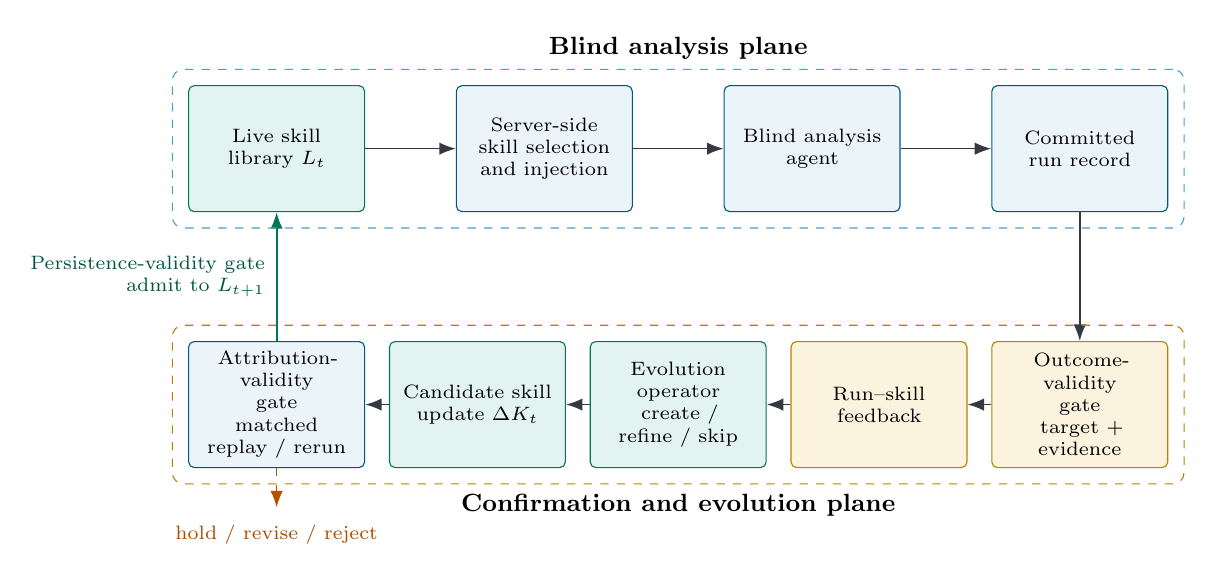
\begin{tikzpicture}[
    box/.style={draw=EvoBlue!75!black, rounded corners=2pt, align=center,
                minimum height=16mm, text width=20mm, font=\scriptsize,
                fill=EvoBlue!8},
    evidence/.style={box, draw=EvoOrange!80!black, fill=EvoOrange!13},
    state/.style={box, draw=EvoGreen!75!black, fill=EvoGreen!11},
    arrow/.style={-{Latex[length=2.1mm]}, line width=0.55pt, draw=EvoDark},
    admitarrow/.style={-{Latex[length=2.1mm]}, line width=0.7pt,
                      draw=EvoGreen!75!black},
    rejectarrow/.style={-{Latex[length=2.1mm]}, line width=0.6pt,
                       draw=EvoRed!85!black, dashed}
]
\node[state] (live) at (0,1.7) {Live skill\\library $L_t$};
\node[box] (select) at (3.4,1.7) {Server-side\\skill selection\\and injection};
\node[box] (agent) at (6.8,1.7) {Blind analysis\\agent};
\node[box] (archive) at (10.2,1.7) {Committed\\run record};

\node[box] (gate) at (0,-1.55) {Attribution-validity\\gate\\matched replay / rerun};
\node[state] (candidate) at (2.55,-1.55) {Candidate skill\\update $\Delta K_t$};
\node[state] (evolve) at (5.1,-1.55) {Evolution\\operator\\create / refine / skip};
\node[evidence] (feedback) at (7.65,-1.55) {Run--skill\\feedback};
\node[evidence] (confirm) at (10.2,-1.55) {Outcome-validity\\gate\\target + evidence};

\draw[arrow] (live) -- (select);
\draw[arrow] (select) -- (agent);
\draw[arrow] (agent) -- (archive);
\draw[arrow] (archive) -- (confirm);
\draw[arrow] (confirm) -- (feedback);
\draw[arrow] (feedback) -- (evolve);
\draw[arrow] (evolve) -- (candidate);
\draw[arrow] (candidate) -- (gate);
\draw[admitarrow] (gate.north) -- node[midway, left=1mm, font=\scriptsize,
    align=right, text=EvoGreen!55!black, fill=white, inner sep=1pt]
    {Persistence-validity gate\\admit to $L_{t+1}$} (live.south);
\draw[rejectarrow] (gate.south) -- ++(0,-5mm)
    node[below=1mm, font=\scriptsize, align=center, text=EvoRed!80!black]
    {hold / revise / reject};

\node[draw=EvoBlue!70, dashed, rounded corners, fit=(live)(select)(agent)(archive),
      inner sep=2mm, label={[font=\small\bfseries]above:Blind analysis plane}] {};
\node[draw=EvoOrange!80!black, dashed, rounded corners,
      fit=(confirm)(feedback)(evolve)(candidate)(gate), inner sep=2mm,
      label={[font=\small\bfseries]below:Confirmation and evolution plane}] {};
\end{tikzpicture}
\caption{Evidence-constrained skill-evolution lifecycle.  Evidence enters only after the
blind answer is committed.  Candidate skills remain isolated while attribution is tested;
admission places a candidate in provisional persistent state, after which it may be
retained, revised, or retired.}
\label{fig:lifecycle}
\end{figure}

\paragraph{Blind analysis plane.}

The controller renders an isolated workspace and records selected skill versions,
injected-prompt hashes, immutable session identifiers, answers, trajectories, and
observed skill-file access.  The agent may inspect visible artifacts but not hidden
answers or validators, ensuring that useful procedures rely on analysis-time features.

\paragraph{Confirmation plane and evidence hierarchy.}

After commitment, target-aware scoring compares file, function, root cause, and evidence
with the case specification.  Source predicates establish code relations; logic harnesses
exercise a state or path; behavioral tests reproduce outputs, timeouts, or state changes;
and sanitizers report memory-safety failures.  These classes validate outcomes, not skill
contribution, and derived skills retain their limitations.

\subsection{Candidate construction, admission, and guarded persistence}

\paragraph{Feedback and candidate construction.}

The post-run record links actual exposure to outcome, component scores, confirmation,
identity flags, and a compact trajectory assessment.  A per-skill bundle preserves
lineage while the service refines, creates, or skips.  Candidates receive a content hash
and separate evaluation because summaries can preserve incidental cues.

\paragraph{Validation, admission, and later reuse.}

Candidates remain isolated for replay or rerun.  Jobs retain evidence, cases, policy,
thresholds, candidate/baseline outcomes, and a terminal decision.  Source replay detects
immediate regression; held-out and longitudinal evidence is required for transfer and
retention.

\paragraph{Prototype realization.}

The SkillClaw extension implements these stages; Appendix~\ref{app:implementation} maps
them to entry points.

\section{Evaluation Methodology}
\label{sec:methodology}

\subsection{Research questions}

We organize the evaluation around three research questions (RQs).  Together, they test
whether skill evolution has measurable headroom, where its learning signals fail, and
how the proposed lifecycle operates in practice:
\begin{description}[leftmargin=1.2cm,style=nextline]
    \item[RQ1.] Does procedural skill content materially change correct-target
    localization and attraction to dangerous decoys, creating measurable opportunity
    for skill evolution under blind execution?
    \item[RQ2.] Which apparently successful runs or refinements are unsafe evolution
    signals because of leakage, target mismatch, or specific detail that fails to
    discriminate the intended target?
    \item[RQ3.] How does the evidence-constrained lifecycle transform confirmed runs into
    governed candidates, and what additional evidence is required to establish candidate
    contribution and persistent transfer?
\end{description}

RQ1 therefore tests skill sensitivity, RQ2 identifies unsafe learning signals, and RQ3
examines the governed path from a run to the skill library.  Skill assignment is fixed
throughout the evaluation, so retrieval quality, confirmation-class effects, and
admission thresholds remain outside the comparison.

\subsection{Benchmark scope and provenance}

\paragraph{Benchmark composition.}

The packaged benchmark comprises 27 case specifications.  Of these, 25 form the
evaluated registry: five source-code cases used for external confirmation and twenty
firmware cases.  The other two cases are excluded.  The strongest accepted evidence for the Exiv2
case reaches only an intermediate path, while the F9K1122 set-password case duplicates
another binary-level case and names a target absent from the visible artifact.
The controlled snapshot described below contains 17 of the 20 registry firmware cases;
the other three remain outside this frozen comparison.

\paragraph{Disclosure provenance.}

A post-run audit mapped 18 of 19 previously empty firmware CVE fields; the invalid
F9K1122 duplicate remained unmapped.  This metadata-only backfill occurred after
execution and was never exposed to the agent.  Reporter aliases link 16 records to two
author-team members and one to an external reporter; one record has no listed reporter.
\emph{System-assisted discovery} means that the workflow contributed to analysis, not
that the agent acted autonomously or that human and agent contributions were quantified.

\paragraph{Frozen evaluation snapshot.}

The fixed snapshot contains 17 firmware cases: three command injections, thirteen
buffer overflows, and one path-traversal/authentication-bypass target across six
device/model groups.  Two F9K1122 near-pairs lack an observable basis for function-level
disambiguation in the frozen agent-visible interface and are reported separately.  The primary
analysis therefore covers 15 cases repeated three times per condition (45 runs each).

Commits \texttt{01f5830} and \texttt{8186f34} fix the protocol and leakage cleanup; the
\texttt{plan11\_frozen} archive contains all 153 scheduled runs.
Table~\ref{tab:benchmark_layers} summarizes how each evidence group supports the three
research questions.

\begin{table}[t]
\centering
\caption{Evidence groups used to evaluate the skill-evolution lifecycle.}
\label{tab:benchmark_layers}
\tableformat
\begin{tabularx}{\textwidth}{L{0.28\textwidth} Y L{0.23\textwidth}}
\toprule
\thead{Evidence group (size)} & \thead{Measurement purpose} & \thead{Role in the evolution study} \\
\midrule
Controlled firmware evaluation (17 cases; 153 runs) & Compare no skill, generic guidance, and constructed case-specific guidance & Establish that procedural content changes blind analysis \\
Leakage-control rerun (14 cases; 84 runs) & Document outcomes after answer-bearing skill content was removed & Identify contaminated evolution signals \\
F9K1122 separable-cue diagnostic (2 targets; 10 runs) & Test refinement when observable cues separate handlers & Positive cue-separability diagnostic \\
FH451 overlapping-cue diagnostic (5 targets; 30 runs) & Test the same refinement in a dense handler region & Negative cue-overlap diagnostic \\
External-confirmation suite (5 source-code cases) & Exercise sanitizer-, behavior-, and logic-backed evidence & Filter outcome-valid experience \\
Lifecycle decision archive (94 decisions) & Record generation, comparison, rejection, and admission paths & Observe governed candidate transitions \\
\bottomrule
\end{tabularx}
\end{table}

The first four groups support performance comparisons or targeted diagnostics.  The
confirmation suite instead exercises available evidence classes, while the lifecycle
archive documents that governed state transitions were executed; neither constitutes
an additional controlled performance experiment.

\subsection{Blind execution and skill conditions}

The remote agent receives a prepared workspace and objective but not CVE identifiers,
ground truth, proof-of-concept artifacts, solution-bearing paths, or validators.  The
controlled firmware runs were executed on August 20, 2026; all conditions used the hosted
model label \texttt{deepseek-v4-flash}.  The 153-run controlled evaluation uses three
repetitions per case--condition pair.
The server records skill versions, prompt hashes, session lineage, and observed skill-file
access.  These records make the exposure reconstructable, but they do not by themselves
establish causality.

The three conditions are:
\begin{itemize}[leftmargin=*]
    \item \textbf{No skill:} no task skill is injected.
    \item \textbf{Generic guidance:} the server injects broad Common Gateway Interface
    (CGI) or Executable and Linkable Format (ELF) triage guidance that does not identify
    a target handler.
    \item \textbf{Constructed case-specific guidance (experimental upper bound):}
    guidance constructed post hoc from the expected analysis route for each case, then
    stripped of target names, device identifiers, and direct answer cues.  It is an
    experimental instrument, not an evolved live skill.
\end{itemize}

An earlier 84-run rerun uses two repetitions per case--condition pair and documents
leakage repair.  After answer-bearing text was removed,
the case-specific condition produced 10/28 hits ($35.7\%$), compared with 39/40
($97.5\%$) in an earlier contaminated configuration.  Because the evaluated cases and
denominators also changed, this contrast diagnoses leakage risk rather than estimating
the removal effect or the RQ1 effect.

\subsection{Outcomes, scoring, and evidence}

The primary outcome is target localization:
\begin{itemize}[leftmargin=*]
    \item \textbf{YES}: the answer names the intended vulnerable target;
    \item \textbf{DECOY}: the answer identifies a known dangerous but target-mismatched path; and
    \item \textbf{NO}: neither the intended target nor a designated decoy is localized.
\end{itemize}

For paper reporting, a post-archive identity audit normalizes the archived label
\path{fromSetCfm} to \path{formSetCfm}, the symbol visible in the artifact, and otherwise
requires exact handler-token matches.  Thus, for example, \path{formWrlclientSet} does
not count as \path{WrlclientSet}.  The audit changes
one primary case-specific-guidance run from NO to YES; historical component scores remain archived
and are used only descriptively.

A secondary 0--10 score combines case-specific predicates for the file, function, root
cause, and supporting evidence.  Identity flags prevent high-scoring decoys from
becoming positive feedback.  Nevertheless, YES/DECOY/NO remains the primary outcome
because scores are not assumed to be comparable across targets.  The confirmation schema distinguishes source-,
logic-, behavior-, and sanitizer-backed evidence; firmware localizations do not imply
equivalent runtime support.

\subsection{Statistical reporting}

Because repetitions within a case are dependent, we emphasize counts and effect sizes.
Case-cluster bootstrap intervals resample the 15 cases while retaining all within-case
runs (200,000 samples; seed \texttt{20260825}); they describe this case set rather than
a broader population.  Because several cases also share device models and firmware
artifacts, a separate sensitivity analysis groups the cases into six device/model
clusters.  This second analysis checks whether the direction depends on treating targets
from the same group as independent cases; it is not used for population inference.

\section{Results and Analysis}
\label{sec:results}

\subsection{Procedural content creates headroom for skill evolution (RQ1)}

The controlled evaluation contains 153 runs.  After separating the 18 near-pair runs,
Table~\ref{tab:frozen_results} reports the remaining 135 runs in the primary analysis.
Constructed case-specific guidance produces 22/45 correct-target localizations ($48.9\%$),
compared with 5/45 ($11.1\%$) for generic guidance and 3/45 ($6.7\%$) without a skill.
The case-cluster bootstrap difference is $+42.2$ percentage points relative
to no skill (bootstrap $95\%$ interval: $[24.4, 62.2]$) and $+37.8$ points relative to
generic guidance ($[22.2, 55.6]$).  Generic guidance exceeds no skill by only $4.4$ points, with an
interval spanning zero ($[-6.7, 20.0]$).

The device/model-group sensitivity analysis preserves the same direction.  Case-specific
guidance exceeds no skill in all six groups, and exceeds generic guidance in five while
tying it in F9K1122.  By contrast, generic guidance improves on no skill only in
F9K1122, is worse in F453, and ties in the other four groups.  The aggregate case-specific
effect is therefore not attributable to a single device/model group.

\begin{table}[t]
\centering
\caption{Primary controlled firmware evaluation after the target-identity audit: 15
cases and three runs per case--condition pair.}
\label{tab:frozen_results}
\compacttable
\setlength{\tabcolsep}{3.5pt}
\begin{tabular}{lrrrrr}
\toprule
\thead{Condition} & \thead{Runs} & \thead{Correct, $n$ (\%)} & \thead{Decoy, $n$ (\%)} & \thead{No finding, $n$ (\%)} & \thead{Archived mean} \\
\midrule
No skill & 45 & 3 (6.7) & 28 (62.2) & 14 (31.1) & 3.92 \\
Generic guidance & 45 & 5 (11.1) & 24 (53.3) & 16 (35.6) & 3.99 \\
\textbf{Case-specific guidance} & \textbf{45} & \textbf{22 (48.9)} & \textbf{2 (4.4)} & \textbf{21 (46.7)} & \textbf{6.20} \\
\bottomrule
\end{tabular}
\end{table}

\begin{figure}[H]
\centering
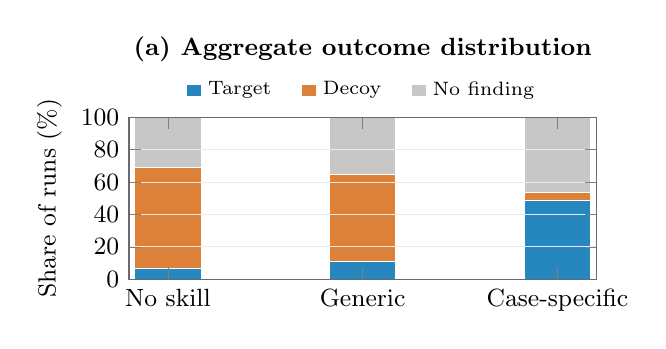
\begin{tikzpicture}
\begin{axis}[
    width=0.62\textwidth,
    height=0.30\textwidth,
    ybar stacked,
    bar width=24pt,
    ymin=0,
    ymax=100,
    ylabel={Share of runs (\%)},
    symbolic x coords={none,generic,upper},
    xtick=data,
    xticklabels={No skill,Generic,Case-specific},
    x tick label style={font=\small,align=center},
    tick label style={font=\small},
    label style={font=\small},
    title={(a) Aggregate outcome distribution},
    title style={font=\small\bfseries,at={(0.5,1.18)},anchor=south},
    legend style={font=\scriptsize,draw=none,at={(0.5,1.04)},anchor=south,
                  legend columns=3,/tikz/every even column/.append style={column sep=3mm}},
    legend image code/.code={\draw[#1] (0cm,-0.08cm) rectangle (0.20cm,0.08cm);},
    axis line style={EvoDark!75},
    ymajorgrids=true,
    grid style={EvoGray!18},
    axis on top,
]
\addplot[fill=EvoBlue!85,draw=white,line width=0.4pt]
    coordinates {(none,6.6667) (generic,11.1111) (upper,48.8889)};
\addplot[fill=EvoRed!78,draw=white,line width=0.4pt]
    coordinates {(none,62.2222) (generic,53.3333) (upper,4.4444)};
\addplot[fill=EvoGray!48,draw=white,line width=0.4pt]
    coordinates {(none,31.1111) (generic,35.5556) (upper,46.6667)};
\legend{Target,Decoy,No finding}
\end{axis}
\end{tikzpicture}

\vspace{2mm}

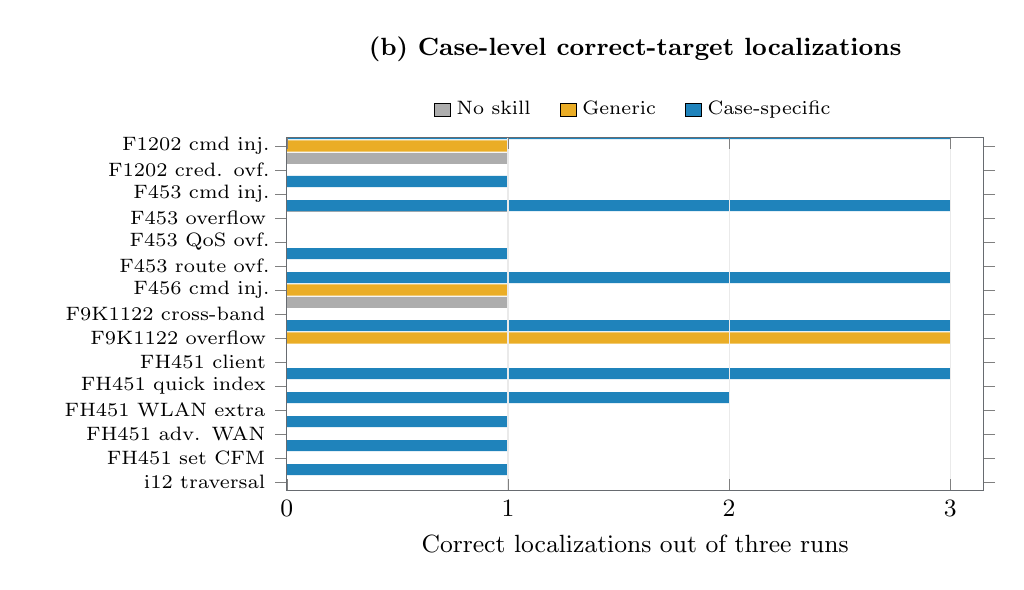
\begin{tikzpicture}
\begin{axis}[
    width=0.86\textwidth,
    height=0.50\textwidth,
    xbar,
    xmin=0,
    xmax=3.15,
    xtick={0,1,2,3},
    xlabel={Correct localizations out of three runs},
    symbolic y coords={
        i12,fhset,fhwan,fhextra,fhquick,fhclient,
        f9ovf,f9cross,f456,f453route,f453qos,f453ovf,f453cmd,f1202cred,f1202cmd
    },
    ytick=data,
    yticklabels={
        i12 traversal,FH451 set CFM,FH451 adv. WAN,FH451 WLAN extra,
        FH451 quick index,FH451 client,F9K1122 overflow,F9K1122 cross-band,
        F456 cmd inj.,F453 route ovf.,F453 QoS ovf.,F453 overflow,
        F453 cmd inj.,F1202 cred. ovf.,F1202 cmd inj.
    },
    y tick label style={font=\scriptsize,text width=29mm,align=right},
    x tick label style={font=\small},
    label style={font=\small},
    title={(b) Case-level correct-target localizations},
    title style={font=\small\bfseries,at={(0.5,1.14)},anchor=south},
    legend style={font=\scriptsize,draw=none,at={(0.5,1.02)},anchor=south,
                  legend columns=3,/tikz/every even column/.append style={column sep=3mm}},
    legend image code/.code={\draw[#1] (0cm,-0.08cm) rectangle (0.20cm,0.08cm);},
    axis line style={EvoDark!75},
    xmajorgrids=true,
    grid style={EvoGray!18},
    enlarge y limits=0.025,
    axis on top,
]
\addplot[fill=EvoGray!70,draw=none,bar width=4pt,bar shift=-4.5pt] coordinates {
    (0,i12) (0,fhset) (0,fhwan) (0,fhextra) (0,fhquick) (0,fhclient)
    (0,f9ovf) (0,f9cross) (1,f456) (0,f453route) (0,f453qos) (0,f453ovf)
    (1,f453cmd) (0,f1202cred) (1,f1202cmd)
};
\addplot[fill=EvoOrange!85,draw=none,bar width=4pt,bar shift=0pt] coordinates {
    (0,i12) (0,fhset) (0,fhwan) (0,fhextra) (0,fhquick) (0,fhclient)
    (3,f9ovf) (0,f9cross) (1,f456) (0,f453route) (0,f453qos) (0,f453ovf)
    (0,f453cmd) (0,f1202cred) (1,f1202cmd)
};
\addplot[fill=EvoBlue!88,draw=none,bar width=4pt,bar shift=4.5pt] coordinates {
    (1,i12) (1,fhset) (1,fhwan) (2,fhextra) (3,fhquick) (0,fhclient)
    (3,f9ovf) (0,f9cross) (3,f456) (1,f453route) (0,f453qos) (3,f453ovf)
    (1,f453cmd) (0,f1202cred) (3,f1202cmd)
};
\legend{No skill,Generic,Case-specific}
\end{axis}
\end{tikzpicture}

\vspace{1mm}

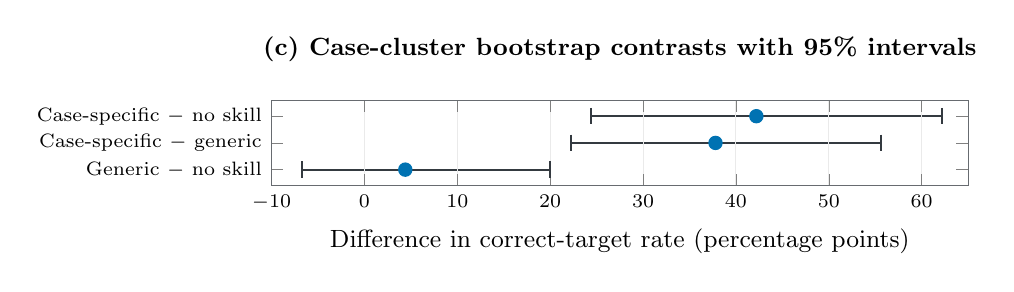
\begin{tikzpicture}
\begin{axis}[
    width=0.86\textwidth,
    height=0.22\textwidth,
    xmin=-10,
    xmax=65,
    xtick={-10,0,10,20,30,40,50,60},
    xlabel={Difference in correct-target rate (percentage points)},
    symbolic y coords={gennone,upgen,upnone},
    ytick=data,
    yticklabels={Generic $-$ no skill,Case-specific $-$ generic,Case-specific $-$ no skill},
    y tick label style={font=\scriptsize},
    x tick label style={font=\scriptsize},
    label style={font=\small},
    title={(c) Case-cluster bootstrap contrasts with 95\% intervals},
    title style={font=\small\bfseries,at={(0.5,1.14)},anchor=south},
    axis line style={EvoDark!75},
    xmajorgrids=true,
    grid style={EvoGray!18},
    enlarge y limits=0.30,
    axis on top,
]
\addplot[EvoGray!75,dashed,line width=0.6pt]
    coordinates {(0,gennone) (0,upgen) (0,upnone)};
\addplot[EvoDark,line width=0.75pt,mark=|,mark size=3pt]
    coordinates {(-6.7,gennone) (20.0,gennone)};
\addplot[EvoDark,line width=0.75pt,mark=|,mark size=3pt]
    coordinates {(22.2,upgen) (55.6,upgen)};
\addplot[EvoDark,line width=0.75pt,mark=|,mark size=3pt]
    coordinates {(24.4,upnone) (62.2,upnone)};
\addplot[only marks,mark=*,mark size=2.4pt,EvoBlue] coordinates {
    (4.4,gennone) (37.8,upgen) (42.2,upnone)
};
\end{axis}
\end{tikzpicture}
\caption{Controlled-evaluation outcomes and effect sizes.  Panel (a) summarizes the
target, designated-decoy, and no-finding outcomes among 45 runs per condition.  Panel
(b) reports correct-target localizations among three runs per primary case.  Panel (c)
shows case-cluster bootstrap contrasts with percentile 95\% intervals.}
\label{fig:frozen_skill_effect}
\end{figure}

Figure~\ref{fig:frozen_skill_effect} shows both the aggregate outcome redistribution and
its case-level heterogeneity.  Decoys fall from 28 without a skill and 24 with generic
guidance to two under case-specific guidance.  This redistribution is consistent with a
change in path selection rather than merely in answer phrasing.  However, 21/45
case-specific-guidance runs remain classified as NO.

The case-specific guidance reaches 3/3 YES on five targets and 0/3 on four others, with partial
success elsewhere.  Its benefit therefore depends on cues being both observable and
discriminative, not on uniform target improvement.

Generic guidance remains close to no skill and its YES-rate interval spans zero: topical
relevance alone does not supply a disambiguating procedure.

For the two separately reported near-pairs, YES counts are 1/6 without a skill and 0/6
under both guidance conditions.

\subsection{Unsafe evolution signals (RQ2)}

Having established that procedural content can change behavior, RQ2 asks when such
changes provide unsafe inputs to persistent skill updates.  We examine three sources:
target mismatch, answer leakage, and specificity that does not actually discriminate
among candidate targets.

\subsubsection{Target mismatch: a plausible decoy can receive a high partial score}

For F453 command injection, only two of 15 development runs localized the intended
\texttt{formWriteFacMac} handler, whereas ten chose the salient
\texttt{formexeCommand} decoy.  Some of these decoys nevertheless scored 8.0 under the
earlier component metric.
The \texttt{function\_identity\_miss} flag now separates vulnerability-class from
target-identity correctness.  These diagnostic runs are not part of the RQ1 denominator.

Such a confirmed alternate finding may still be useful in an open audit, but it must be
scored separately from success on the controlled target.

\subsubsection{Answer leakage creates contaminated evolution signals}

After direct target and device cues were removed, the 84-run rerun produced correct-target
rates of $3.6\%$, $14.3\%$, and $35.7\%$ for no skill, generic, and case-specific guidance,
with 9, 12, and 1 decoys.  The cleaned case-specific condition localized the correct target
in 10/28 runs, compared with 39/40 in the earlier contaminated configuration.  Because
the case set and denominator also changed, this gap is diagnostic of leakage risk rather
than a matched effect estimate.  This sensitivity is consistent with broader evidence
that duplicate data and nonchronological splits can inflate vulnerability-detection
benchmarks~\cite{primevul}.  The 153-run study supplies the final RQ1 estimate.

\subsubsection{Refinement outcomes depend on cue discriminability}

The targeted diagnostics test whether observable cues can redirect the model away from
a persistent target-mismatched attractor.  Their results provide target-level evidence,
not conclusions about an entire firmware family.
Table~\ref{tab:refinement_diagnostics} summarizes the two cue regimes.

\begin{table}[t]
\centering
\caption{Targeted refinement diagnostics: correct-target localizations under
label-audited target identities with generic and distinguishing guidance.  Denominators
reflect archived, unpaired repetitions.}
\label{tab:refinement_diagnostics}
\tableformat
\begin{tabularx}{\textwidth}{L{0.31\textwidth} C{0.22\textwidth} Y}
\toprule
\thead{Diagnostic target} & \thead{Correct localizations} & \thead{Interpretation} \\
\midrule
F9K1122 \texttt{formCrossBandSwitch} & $0/2 \rightarrow 3/3$ & Unique neighbors dislodge the \texttt{formWISP5G} attractor \\
F9K1122 \texttt{formWlanSetup} & $0/2 \rightarrow 3/3$ & Stable local cues recover the intended handler \\
FH451 five-target aggregate & $7/15 \rightarrow 5/15$ & Overlapping cues do not improve the aggregate and coincide with lower observed success \\
\bottomrule
\end{tabularx}
\end{table}

In F9K1122, separated handler neighborhoods coincide with full localization under the
additional cues; in FH451, overlapping names, neighbors, and parameters coincide with
more redirection to similar handlers.  The observed refinement outcome is therefore
structure-dependent rather than monotonically beneficial.

\paragraph{F9K1122: higher observed success with separable cues.}

Generic guidance repeatedly selected \texttt{formWISP5G} instead of
\texttt{formCrossBandSwitch} or \texttt{formWlanSetup}.  For each target, the observed
count was 0/2 with generic guidance and 3/3 with answer-free neighborhood cues, which
exclude that attractor through visible local structure.

The same study invalidated a set-password case whose target was absent from the visible
binary, distinguishing task unidentifiability from skill failure.

\paragraph{FH451: lower observed success with overlapping cues.}

For five overlapping FH451 targets, label-audited success is 7/15 with generic guidance
and 5/15 with the additional neighborhood cues; the latter condition often redirects the
model to semantically similar neighbors.
Specificity helps only when features reduce the candidate set; dense regions require
stronger evidence such as call graphs, cross-references, or dispatch order.

The identity audit corrects two opposing labeling effects in this diagnostic: normalized
\texttt{formSetCfm} predictions are recognized, while the substring-only
\texttt{formWrlclientSet} prediction is rejected as a match for \texttt{WrlclientSet}.

\subsection{Evidence-constrained candidate governance (RQ3)}

RQ3 moves from identifying unsafe signals to examining how the system governs them.  It
asks how confirmation filters the runs supplied to candidate construction and how the
lifecycle records comparison and terminal admission decisions.

\subsubsection{External confirmation filters outcome-valid experience}

Table~\ref{tab:confirmation_cases} pairs each archived blind outcome with its strongest
available post-run confirmation mechanism.

\begin{table}[H]
\centering
\caption{Archived blind-run outcomes and strongest case-specific confirmation mechanisms.}
\label{tab:confirmation_cases}
\tableformat
\begin{tabularx}{\textwidth}{L{0.16\textwidth} L{0.15\textwidth} C{0.07\textwidth} C{0.09\textwidth} C{0.12\textwidth} Y}
\toprule
\thead{Case} & \thead{Public CVE} & \thead{Score} & \thead{Target found} & \thead{Evidence met} & \thead{Strongest confirmation} \\
\midrule
GIFLIB 5.1.2 & CVE-2016-3977 & 8/10 & Yes & Yes & Sanitizer-backed crash \\
libarchive 3.8.0 & CVE-2025-60753 & 10/10 & Yes & Yes & Timeout-backed behavior \\
libxml2 2.9.4 & CVE-2017-8872 & 8/10 & Yes & Yes & Logic-harness path \\
tcpdump 4.9.1 & CVE-2017-13031 & 10/10 & Yes & Yes & Packet-processing behavior \\
tcpdump 4.9.1 & CVE-2018-14469 & 2/10 & No & No & Payload-length behavior (available) \\
\bottomrule
\end{tabularx}
\end{table}

Four runs satisfy both the target and evidence requirements.  The second tcpdump run
does not, even though a behavioral validator is available.  Validator availability must
therefore be distinguished from success by the blind run itself.

\subsubsection{Lifecycle archive documents governed candidate transitions}

The archive contains 94 decisions (12 published, 82 rejected).  A separate audit of 119
admission and validation jobs found 21 rerun jobs that should have terminated as rejected
but lacked terminal state; the audit settled all 21 as rejected.
Table~\ref{tab:lifecycle_archive} keeps these denominators separate.

\begin{table}[H]
\centering
\caption{Lifecycle archive and settlement-audit snapshots; the denominators differ.}
\label{tab:lifecycle_archive}
\tableformat
\begin{tabularx}{\textwidth}{L{0.20\textwidth} L{0.34\textwidth} Y}
\toprule
\thead{Snapshot} & \thead{Population and outcome} & \thead{What the snapshot documents} \\
\midrule
Decision archive & 94 records: 12 published; 82 rejected & Publication and rejection paths executed under mixed historical regimes \\
Settlement audit & 119 jobs: 21 stalled jobs settled as rejected; 0 unresolved afterward & Terminal-state guard removed a pending-job failure mode \\
\bottomrule
\end{tabularx}
\end{table}

In one end-to-end trace, \path{firmware2-wireless-seed-20260812a}, a weak exposed skill
produced feedback, a queued revision, and matched replay.  Candidate and baseline both
scored 1.0, so strict improvement rejected the candidate (Figure~\ref{fig:candidate_episode}).

\begin{figure}[H]
\centering
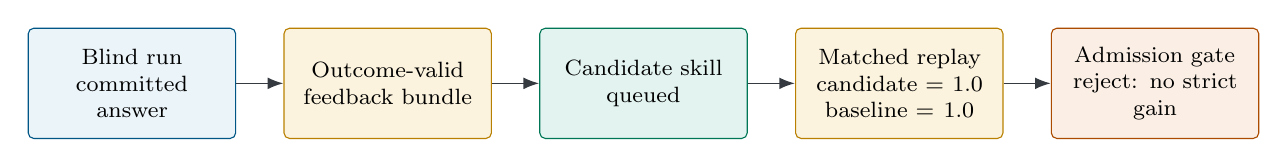
\begin{tikzpicture}[
    node distance=6mm,
    stagebox/.style={draw=EvoBlue!75!black, rounded corners=2pt, align=center,
                 minimum height=14mm, text width=24mm, font=\footnotesize,
                 fill=EvoBlue!8},
    evidence/.style={stagebox, draw=EvoOrange!80!black, fill=EvoOrange!13},
    candidatebox/.style={stagebox, draw=EvoGreen!75!black, fill=EvoGreen!11},
    decision/.style={stagebox, draw=EvoRed!80!black, fill=EvoRed!10},
    arrow/.style={-{Latex[length=2mm]}, line width=0.6pt, draw=EvoDark}
]
\node[stagebox] (run) {Blind run\\committed\\answer};
\node[evidence, right=of run] (handoff) {Outcome-valid\\feedback bundle};
\node[candidatebox, right=of handoff] (candidate) {Candidate skill\\queued};
\node[evidence, right=of candidate] (replay) {Matched replay\\candidate $=1.0$\\baseline $=1.0$};
\node[decision, right=of replay] (reject) {Admission gate\\reject: no strict\\gain};

\draw[arrow] (run.east) -- (handoff.west);
\draw[arrow] (handoff.east) -- (candidate.west);
\draw[arrow] (candidate.east) -- (replay.west);
\draw[arrow] (replay.east) -- (reject.west);
\end{tikzpicture}
\caption{Observed candidate-evolution episode.  A blind run produced outcome-valid
feedback, a candidate skill, and a matched replay decision.  Equal candidate and baseline
scores support rejection under the strict-improvement rule; they do not demonstrate
candidate gain.}
\label{fig:candidate_episode}
\end{figure}

Taken together, the snapshots show that generation, validation, rejection, publication,
and settlement were all executed.  Because the records span different historical
regimes, however, they cannot estimate an admission rate or future-task effect.  They
demonstrate the need for terminal governance and baseline-aware replay, while also
showing that confirmation cannot replace matched comparison.

\subsection{Operational context and public-disclosure provenance}

Among 18 valid firmware CVE backfills, public reporter aliases link 16 CVEs to two
author-team members; 15 of the 17 controlled cases belong to this group.  The project-side
mapping classifies those 16 discoveries as system-assisted.  This provenance documents
operational use and public disclosure, while distinguishing the public reporter field
from the project interpretation.  The experiment itself nevertheless remains a
post-disclosure localization study in which CVE metadata is withheld, so it does not
quantify autonomy or causal skill contribution.

\subsection{Summary of research-question findings}

Table~\ref{tab:findings} maps the principal findings back to the three validity gates.

\begin{table}[H]
\centering
\caption{Evidence summary and implications for evidence-constrained skill evolution.}
\label{tab:findings}
\tableformat
\begin{tabularx}{\textwidth}{L{0.17\textwidth} L{0.43\textwidth} Y}
\toprule
\thead{Evolution gate} & \thead{Finding} & \thead{Implication for evolution} \\
\midrule
Outcome (RQ1--RQ2) & Case-specific guidance audited to remove direct answer cues increases correct-target localization and reduces decoy attraction; leakage and target mismatch can inflate apparent success & Outcome labels must preserve blindness, target identity, and evidence strength \\
Attribution (RQ1--RQ3) & Controlled skill conditions change aggregate behavior, but confirmation and replay alone do not isolate the responsible procedure & Skill sensitivity is observed; candidate contribution requires matched comparison \\
Persistence (RQ2--RQ3) & Distinguishing cues localize separable F9K1122 targets but coincide with lower observed success in the FH451 aggregate; candidates reach rejection and publication states & Reuse depends on task structure, and admission is not equivalent to long-term utility \\
\bottomrule
\end{tabularx}
\end{table}

\section{Discussion and Limitations}
\label{sec:discussion}

\subsection{What the evidence establishes about skill evolution}

The controlled study establishes \emph{skill sensitivity}: answer-audited procedural
content changes localization and decoy attraction.  Because the case-specific guidance
is manually constructed, it measures procedural headroom, not constructor quality.

Evidence is not attribution: confirmation establishes what was found, while matched
counterfactuals are needed to isolate the skill from the base model.  Similar scores can
also hide different behavioral signatures~\cite{trajectoryprograms}.  Attribution is not
persistence either: the F9K1122/FH451 contrast shows why source-case gains require
held-out and longitudinal checks.

The three gates therefore fail independently.  Strong sanitizer evidence can support an
outcome without identifying the responsible skill, and a reproducible candidate gain can
still encode an artifact-specific heuristic that should not persist.

Relative to executable, reconstruction-, replay-, or verifier-based systems
~\cite{asi,mindskill,skillcommit,coevoskills,trace2skilleda,skillforge} and EvoHunt
~\cite{evohunt}, our evidence supports a security-specific formulation, content
sensitivity, and an operational governance path---not superior transfer.  The distinction
is the coupling of target identity and heterogeneous vulnerability evidence to
attribution and retention.

\subsection{Failure modes and library governance}

A selectable library can fail in selection, content, or evolution: it may retrieve the
wrong procedure, encode a brittle rule, or persist misleading evidence.  Run--skill
linkage and identity diagnostics separate these causes, although fixed assignment does
not measure selection quality.  Candidate/live isolation permits rejection before
publication, while longitudinal evidence supports later revision, demotion, or retirement.

This decomposition also guides remediation: selection errors call for descriptors or
retrieval changes, content errors for procedural revision, and evolution errors for
stricter evidence and admission policies.

\subsection{Implications for vulnerability-analysis benchmarks}

Known-vulnerability cases offer target identity and confirmation but require leakage and
identifiability audits.  Alternate findings should remain separate from controlled-target
success.  Benchmarks should therefore retain exact exposure, measure target-correct
outcomes, and separate source replay from held-out persistence; our suite implements the
first two and isolates replay state, while held-out persistence remains future work.

The target label should not suppress open-ended findings.  It should preserve two records:
whether the controlled target was found and whether the run uncovered another independently
supported vulnerability.

\subsection{Threats to validity}
\label{sec:threats}

\paragraph{Case scale and dependence.}
The primary result covers 15 cases with three dependent repetitions; cluster-bootstrap
intervals and the six-group sensitivity analysis do not support broad population inference.

\paragraph{Single model and agent configuration.}
One model and harness may not represent different analysis priors or instruction following.

\paragraph{Answer leakage.}
Identifiers, files, comments, artifacts, or skills can leak answers; the cleaned rerun
documents the threat but cannot prove its absence.

\paragraph{Pretraining contamination.}
Post-disclosure cases may remain in model parameters or provider retrieval; we control
the visible interface, not pretraining novelty.

\paragraph{Benchmark curation.}
One case was invalidated, two near-pairs separated, and two FH451 labels corrected,
limiting older aggregates.

\paragraph{Evidence heterogeneity.}
Runtime confirmation belongs to the source suite; firmware results are largely static,
and evidence classes are not causally compared.

\paragraph{Attribution precision.}
Scores detect wrong or unsupported answers but do not decompose skill contribution.

\Needspace{7\baselineskip}
\paragraph{Contemporary evolution baselines.}
The study does not directly compare learned candidates with contemporary systems
~\cite{asi,mindskill,skillcommit,coevoskills,trace2skilleda,skillforge,evohunt}; such
claims require matched held-out evaluation.

\paragraph{Lifecycle archive comparability.}
The 94 decisions span mixed regimes and support execution, not policy comparison or an
overall admission rate.

\paragraph{Service and artifact reproducibility.}
Hosted models may change, and replication depends on released prompts, artifacts,
configurations, and code.

\paragraph{Discovery attribution.}
Reporter records establish disclosure provenance, not human--agent contribution or yield.

\paragraph{External validity.}
The diagnostics do not establish generality across models, ecosystems, or open discovery.

\subsection{Ethical scope}
\label{sec:ethics}

Experiments use packaged known vulnerabilities and archived artifacts in isolated
workspaces; no undisclosed vulnerability or production targeting is reported.  The work
is defensive.  Appendix aliases are public CVE strings used for provenance, and the
project-side author mapping is reported with permission.

\subsection{Future work}
\label{sec:agenda}

The next evaluation should freeze candidates and lineage from designated source runs,
then compare no skill, a fixed baseline, and the candidate on held-out blind cases with
an immutable runner.  Baselines should cover executable/reconstructed skills, replay or
isolated verification, longitudinal tracking, and EvoHunt's global playbook.

This design would directly estimate candidate contribution and transfer while preventing
evaluation feedback from altering either the candidate or the live library.

Longitudinal governance should instrument retrieval, trajectory change, and later
evidence to distinguish selection from content errors and support demotion or retirement.
Broader benchmarks should add executable source and firmware confirmation, separate new
findings from target-conditioned outcomes, control memorization by time or artifact, and
evaluate multiple models.

\section{Conclusion}
\label{sec:conclusion}

This paper studies how blind vulnerability-analysis agents can evolve reusable skills
from verified experience.  The proposed lifecycle connects blind execution, auditable
skill exposure, target-aware and heterogeneous confirmation, run-derived feedback,
candidate creation or refinement, replay or rerun validation, and governed publication
into a live library.  Outcome, attribution, and persistence validity act as gates on this
evolution process: they determine which runs may teach, whether a candidate changed the
result, and whether the learned procedure should remain available to future analyses.

The controlled study establishes the premise that makes evolution worthwhile:
procedural guidance audited to remove direct answer cues substantially increases correct-target localization
and reduces dangerous-decoy attraction.  It also identifies signals that naive evolution
would mishandle.  Leakage can turn answer retrieval into apparent learning, a confirmed
alternate vulnerability can reinforce the wrong target, and additional specificity can
localize separable F9K1122 targets while coinciding with lower success in the overlapping
FH451 region.

The external-confirmation suite demonstrates multiple independent evidence classes, and
the lifecycle archive records candidate construction, comparison, rejection,
publication, and terminal-state settlement.  Project-side provenance further links the
workflow to 16 public CVEs reported by two author-team members and classifies the
corresponding discoveries as system-assisted, recording use beyond an externally curated
benchmark.  Taken together, these
elements provide an evidence-constrained formulation and implementation of vulnerability-analysis skill
evolution, together with an empirical account of why evolution signals must preserve
blindness, target identity, causal comparison, and transfer.

Overall, the study defines, implements, and exercises an auditable, evidence-governed
lifecycle for evolving vulnerability-analysis skills.  Matched candidate-on/candidate-off
experiments, held-out transfer, and longitudinal retention provide the next evaluation
layer for measuring evolution quality and extending the implemented lifecycle toward
cumulative procedural learning for vulnerability-analysis agents.

\appendix
\section{Implementation Mapping}
\label{app:implementation}

Table~\ref{tab:implementation_map} maps the evolution method to the principal entry points
used by the implementation.  The mapping supports implementation traceability; exact
reproducibility additionally requires the corresponding code, configurations, prompts,
and artifacts.  The conceptual formulation does not depend on these particular file or
directory names.

\begin{table}[H]
\centering
\caption{Prototype stages, implementation entry points, and persisted outputs.}
\label{tab:implementation_map}
\compacttable
\begin{tabularx}{\textwidth}{L{0.22\textwidth} L{0.41\textwidth} Y}
\toprule
\thead{Stage} & \thead{Principal entry points} & \thead{Persisted output} \\
\midrule
Skill exposure and session archive &
\path{skillclaw/skill_manager.py};
\path{skillclaw/api_server.py} &
selected versions, prompt hash, session/segment lineage, observed skill access \\
Blind task preparation and execution &
\path{evaluation/utils/prepare_blind_workspace.py};
\path{evaluation/runs/run_remote_case.py} &
isolated workspace, raw answer, run metadata \\
Scoring and confirmation &
\path{evaluation/runs/score_case_output.py};
\path{evaluation/confirmation/core.py} &
target-aware score, validator result, evidence class \\
Outcome archival and feedback &
\path{evaluation/postprocess/finalize_record.py};
\path{evaluation/reporting/feedback/build_feedback_bundle.py} &
finalized outcome, selected-skill linkage, per-skill feedback bundle \\
Candidate construction and queueing &
\path{evolve_server/engines/workflow.py} &
candidate hash, source lineage, replay cases, validation job \\
Replay, rerun, and settlement &
\path{skillclaw/replay_gate_worker.py};
\path{skillclaw/validation_worker.py} &
candidate/baseline results, gate policy, terminal admission decision \\
Governed skill state &
\path{skillspace/live/}; \path{skillspace/share/} &
live skills separated from candidate, rejected, and history artifacts \\
\bottomrule
\end{tabularx}
\end{table}

\section{Firmware Evaluation Case Set}
\label{app:frozen_cases}

Table~\ref{tab:frozen_case_list} records the 17-case firmware evaluation set.  Short keys
match the archived experiment report, while CVE identifiers come from the post-run
provenance audit described in Section~\ref{sec:methodology}.  ``Primary'' means the case
contributes three runs per condition to the 15-case function-level primary analysis;
``near-pair'' means it is reported separately under the controlled protocol.

\begin{table}[H]
\centering
\caption{Cases in the 153-run controlled firmware evaluation.}
\label{tab:frozen_case_list}
\compacttable
\begin{tabularx}{\textwidth}{L{0.24\textwidth} L{0.16\textwidth} L{0.13\textwidth} L{0.19\textwidth} Y}
\toprule
\thead{Archived case key} & \thead{Public CVE} & \thead{Device / model} & \thead{Vulnerability class} & \thead{Reporting} \\
\midrule
\path{f1202-cmdinject} & CVE-2024-30637 & Tenda F1202 & CGI command injection & primary \\
\path{f1202-credential-overflow} & CVE-2025-7527 & Tenda F1202 & stack overflow / credential decoding & primary \\
\addlinespace[2pt]
\path{f453-cmdinject} & CVE-2026-4554 & Tenda F453 & CGI command injection & primary \\
\path{f453-overflow} & CVE-2026-3273 & Tenda F453 & stack overflow & primary \\
\path{f453-qossetting-overflow} & CVE-2026-3378 & Tenda F453 & stack overflow & primary \\
\path{f453-routestatic-overflow} & CVE-2026-3166 & Tenda F453 & stack overflow & primary \\
\addlinespace[2pt]
\path{f456-cmdinject} & CVE-2026-7102 & Tenda F456 & CGI command injection & primary \\
\addlinespace[2pt]
\path{f9k1122-crossband-overflow} & CVE-2026-5042 & Belkin F9K1122 & stack overflow & primary \\
\path{f9k1122-overflow} & CVE-2026-4566 & Belkin F9K1122 & stack overflow & primary \\
\path{f9k1122-setsystemsettings-overflow} & CVE-2026-5044 & Belkin F9K1122 & stack overflow & near-pair \\
\path{f9k1122-wlansetup-overflow} & CVE-2026-5608 & Belkin F9K1122 & stack overflow & near-pair \\
\addlinespace[2pt]
\path{fh451-WrlclientSet-overflow} & CVE-2026-4535 & Tenda FH451 & stack overflow & primary \\
\path{fh451-formQuickIndex-overflow} & CVE-2026-3679 & Tenda FH451 & stack overflow & primary \\
\path{fh451-formWrlExtraSet-overflow} & CVE-2026-4534 & Tenda FH451 & stack overflow & primary \\
\path{fh451-fromAdvSetWan-overflow} & CVE-2026-3678 & Tenda FH451 & stack overflow & primary \\
\path{fh451-fromSetCfm-overflow} & CVE-2026-3677 & Tenda FH451 & stack overflow; naming inconsistency & primary \\
\addlinespace[2pt]
\path{i12-pathtraversal} & CVE-2026-5849 & Tenda i12 & path traversal / authentication bypass & primary \\
\bottomrule
\end{tabularx}
\end{table}

The provenance audit retains two naming qualifications.  For CVE-2025-7527, the public
record commonly uses \emph{FH1202}, whereas the local execution artifact and archived
case key use \emph{F1202}.  For CVE-2026-3677, public material may use
\texttt{formSetCfm}, whereas the archived case uses \texttt{fromSetCfm}.  The archive
preserves the execution-time identifiers, while paper-level outcome reporting discloses
and applies the \texttt{formSetCfm} normalization rather than changing the record
silently.

The official-record field retained by the audit is \emph{reporter}.
Table~\ref{tab:reporter_provenance} groups the 18 valid firmware CVE backfills by that public
field.  This table covers the evaluated case registry, including the i12 overflow case that
is not part of the 17-case controlled evaluation.  The project-side identity
mapping associates the four LTZ-style aliases with author-team member LTZ and the Jimi
alias with author-team member Jimi.  This mapping documents discovery provenance; it
does not determine author order, affiliation, or degree of automation.

\begin{table}[H]
\centering
\caption{Reporter and author-team provenance for the 18 valid firmware CVE backfills.}
\label{tab:reporter_provenance}
\tableformat
\begin{tabularx}{\textwidth}{L{0.25\textwidth} L{0.24\textwidth} Y}
\toprule
\thead{Public-record reporter} & \thead{Project interpretation} & \thead{Associated CVE records} \\
\midrule
LtzHust (VulDB User) & LTZ; team author; system-assisted & CVE-2026-4554; CVE-2026-3273; CVE-2026-3166; CVE-2026-4566 \\
LtzHust2 (VulDB User) & LTZ; team author; system-assisted & CVE-2026-3378; CVE-2026-5608; CVE-2026-5849 \\
LtzHuster (VulDB User) & LTZ; team author; system-assisted & CVE-2026-7102; CVE-2026-3679; CVE-2026-4534; CVE-2026-3678; CVE-2026-3677; CVE-2026-4535 \\
LtzHuster2 (VulDB User) & LTZ; team author; system-assisted & CVE-2026-5042; CVE-2026-5044 \\
\addlinespace[2pt]
Jimi (VulDB User) & Jimi; team author; system-assisted & CVE-2026-4041 \\
\addlinespace[2pt]
\texttt{panda\_0x1} (VulDB User) & external reporter & CVE-2025-7527 \\
Not listed & provenance unspecified & CVE-2024-30637 \\
\bottomrule
\end{tabularx}
\end{table}

\section{Per-Case Evaluation Outcomes}
\label{app:per_case_results}

Table~\ref{tab:per_case_results} reports the complete primary-case outcome counts behind
Table~\ref{tab:frozen_results}.  Each cell is formatted as YES/DECOY/NO over three runs.
The two near-pair cases remain excluded from this primary analysis and are reported
separately in the main text.

\begin{table}[H]
\centering
\caption{Per-case outcome counts in the controlled evaluation (YES/DECOY/NO).}
\label{tab:per_case_results}
\tableformat
\begin{tabularx}{\textwidth}{L{0.38\textwidth} L{0.16\textwidth} L{0.16\textwidth} Y}
\toprule
\thead{Case key} & \thead{No skill} & \thead{Generic guidance} & \thead{Case-specific guidance} \\
\midrule
\path{f1202-cmdinject} & 1/0/2 & 1/0/2 & 3/0/0 \\
\path{f1202-credential-overflow} & 0/0/3 & 0/0/3 & 0/0/3 \\
\addlinespace[2pt]
\path{f453-cmdinject} & 1/2/0 & 0/2/1 & 1/2/0 \\
\path{f453-overflow} & 0/3/0 & 0/3/0 & 3/0/0 \\
\path{f453-qossetting-overflow} & 0/3/0 & 0/2/1 & 0/0/3 \\
\path{f453-routestatic-overflow} & 0/3/0 & 0/3/0 & 1/0/2 \\
\addlinespace[2pt]
\path{f456-cmdinject} & 1/2/0 & 1/1/1 & 3/0/0 \\
\addlinespace[2pt]
\path{f9k1122-crossband-overflow} & 0/0/3 & 0/0/3 & 0/0/3 \\
\path{f9k1122-overflow} & 0/1/2 & 3/0/0 & 3/0/0 \\
\addlinespace[2pt]
\path{fh451-WrlclientSet-overflow} & 0/3/0 & 0/3/0 & 0/0/3 \\
\path{fh451-formQuickIndex-overflow} & 0/2/1 & 0/1/2 & 3/0/0 \\
\path{fh451-formWrlExtraSet-overflow} & 0/2/1 & 0/2/1 & 2/0/1 \\
\path{fh451-fromAdvSetWan-overflow} & 0/1/2 & 0/3/0 & 1/0/2 \\
\path{fh451-fromSetCfm-overflow} & 0/3/0 & 0/1/2 & 1/0/2 \\
\addlinespace[2pt]
\path{i12-pathtraversal} & 0/3/0 & 0/3/0 & 1/0/2 \\
\bottomrule
\end{tabularx}
\end{table}

\clearpage
\renewcommand{\bibfont}{\small}
\setlength{\bibsep}{1pt plus 0.3ex}
\bibliographystyle{unsrtnat}
\bibliography{references_arxiv_checked}

\end{document}
